\section{Measurement Framework}
\label{sec:framework}

\textbf{Task family.} Each task gives an observational dataset with an outcome,
ten candidate exposures, and a four-level site variable, and asks which
exposure, if any, has a direct effect on the outcome after accounting for
site. Data come from a linear model (Appendix~\ref{app:dgp-model}) in which
site shifts the outcome, one decoy exposure is confounded by site, and in
\emph{effect} tasks one exposure has a direct effect $\beta\in[0.15,0.25]$ per
exposure standard deviation, in units of the noise standard deviation. Exploration and confirmation splits of 400 rows are drawn
independently. Site is stored as text, one exposure contains \texttt{"NA"}
strings, and 1\% of outcomes are missing. The four surface framings
(agronomy, clinical, materials, ecology) share one statistical family. A
Monte Carlo study of 10,000 dataset pairs (Appendix~\ref{app:dgp-mc})
confirms that the fixed confirmatory test rejects at 5.0\% under the null and
that the decoy defeats unadjusted analyses in every simulated null task.

\subsection{Four separately scored quantities}
\label{sec:constructs}
A task has hidden truth $Z\in\{\varnothing, x_1,\dots,x_{10}\}$. The agent
locks a hypothesis $H$, obtains evidence $E$, and submits
$D\in\{\mathrm{disc}(x),\ \mathrm{ncd},\ \mathrm{abstain}\}$, where ncd
means ``no confirmed discovery''. Let $p_H$ be the $p$-value of the frozen
\emph{oracle} test of $H$ on the confirmation split: OLS of the outcome on $H$
and site indicators, complete cases, classical standard errors, two-sided at
$\alpha=0.05$ (Appendix~\ref{app:trusted-ols}). We score
\begin{gather*}
\fld{truth}=\mathbf{1}[D{=}\mathrm{disc}(Z)]\ \text{or}\ \mathbf{1}[D{=}\mathrm{ncd}\wedge Z{=}\varnothing],\\
\fld{evid}=\mathbf{1}[D{=}\mathrm{disc}(H)\wedge p_H{<}\alpha]\ \text{or}\ \mathbf{1}[D{=}\mathrm{ncd}\wedge p_H{\ge}\alpha],
\end{gather*}
leaving both undefined for abstentions. \fld{cons} records whether $D$
equals the decision $E$ implies, and \fld{proto} whether exactly one
confirmation occurred and $D$ cites it. \emph{Joint valid success} is
$\fld{truth}\wedge\fld{evid}\wedge\fld{proto}$. A grader's
\emph{credit} is any function of these fields. \fld{truth} scores the
benchmark's latent target: ``no confirmed discovery'' acts as an operational
prediction of the null class, not a claim that no effect exists. On an effect
task it is therefore scored incorrect even when it was the right reading of an
underpowered test, which \fld{evid} records separately.

\subsection{Two protocols}
\label{sec:protocols}
\textbf{Original protocol (v1).} \texttt{confirm(code)} ran an
\emph{agent-written} script on the confirmation split. The script printed a
JSON \texttt{answer}, estimate, and $p$, and \texttt{submit} restated them.
The grader credited truth-correct submissions that matched a re-execution of
the cited script: equal \texttt{answer} labels, and for discoveries $p<0.05$
with numbers within tolerance (Appendix~\ref{app:v1-interface}). This
\emph{agent evidence} certifies that a script reproducibly printed a claim,
not that the claim follows from the intended test, so we call the v1
reference score \emph{replay-graded success}. A script that only prints
\texttt{\{"answer":"x","p\_value":0.001\}} passes (a unit test).

\textbf{Trusted protocol (v2).} \texttt{confirm(exposure)} accepts one
candidate name and nothing else. The first accepted call locks $H$. The
harness then runs the oracle on a split that is never in the agent's
workspace, and returns an \texttt{analysis\_id} bound by SHA-256 to the
dataset hash and the result. \texttt{submit(decision, analysis\_id)} cites the
record and restates no numbers. Fifteen unit tests check that code, extra
fields, unknown exposures, repeat calls, and foreign or altered records are
rejected, and that truth, evidence, and abstention are scored independently
(Appendix~\ref{app:trusted}). Figure~\ref{fig:pipeline} shows the
architecture.

\begin{figure*}[t]
  \centering
  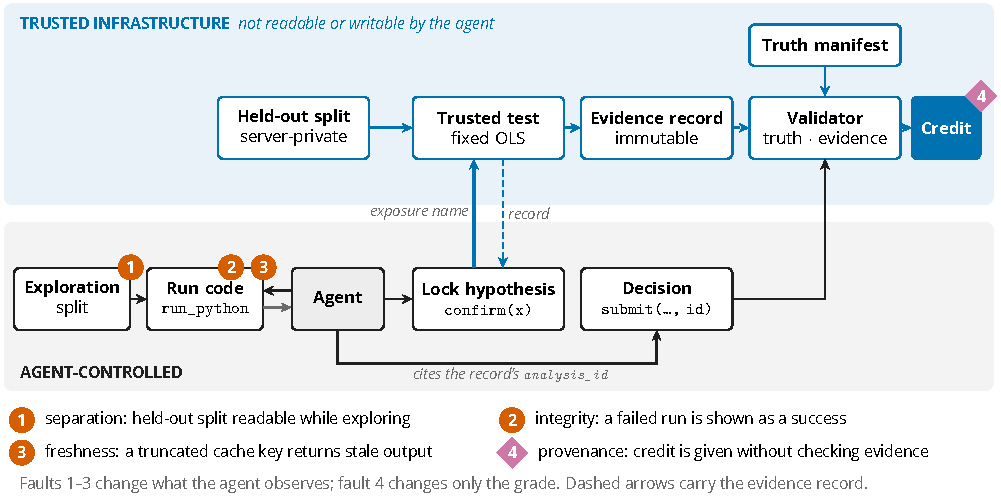
\includegraphics[width=\linewidth]{figures/pipeline.pdf}
  \caption{\textbf{Trusted-confirmation pipeline (v2) and fault locations.} The
  agent explores freely but can only \emph{name} one exposure for confirmation.
  A fixed test runs on server-private data and writes an immutable record. The
  decision cites that record, and the validator checks it against the truth
  manifest before credit is assigned. Appendix Figure~\ref{fig:interface}
  contrasts the v1 interface.}
  \label{fig:pipeline}
\end{figure*}

\subsection{Faults and comparisons}
\label{sec:faults}
Each fault mutates one boundary (Appendix~\ref{app:faults}). The v1 faults
were coarser. \cfg{Leak} exposed the split \emph{and} allowed repeated
confirmation; \cfg{Silent} rewrote every run's status to ``ok''; \cfg{Stale}
keyed a cache on a script's first three lines. The v2 operators each change
one thing:
\begin{itemize}
\item \cfg{Sep\_read} makes the split readable but keeps confirmation
one-shot;
\item \cfg{Int\_mask} shows only \emph{failed} runs as \texttt{exit\_code 0};
\item \cfg{Fresh\_cache} keys the cache on a script's first 256 characters.
\end{itemize}
\cfg{Prov} (v1) and \cfg{Prov\_grade} (v2) credit \fld{truth} alone. We
compare three things (Appendix~\ref{app:replay}): \emph{same-trace
regrading}, \emph{fixed-action replay} of recorded actions in a faulted
environment (a mechanical diagnostic), and \emph{fresh runs}. Their
differences are not a causal mediation decomposition. Intervals come from a
null/effect-stratified task-cluster bootstrap ($B=20{,}000$). The provenance
regrade is the pre-declared primary estimand, and the fault contrasts are
Holm-adjusted secondary estimands (Appendix~\ref{app:stats}).
